In this work we will treat the analysis of the behavior of a viscoelastic fluid using a continuum approximation. We abandon the true molecular character of the fluid in favor of a model which describes the material as continuously distributed throughout the occupied space. We can then subdivide the fluid into infinitesimal fluid elements over which varables such as density and pressure are constant. These same variables are taken to vary continuously with neighboring fluid elements. Combining this approximation with mass and momentum conservation allows us to derive partial differential equations that describe the behavior of a general continuum material. We then combine these with constitutive relations to describe specific materials. We will begin by describing this process for a Newtonian fluid and then extend the model to include viscoelasticity as outlined by Morozov and Spagnolie~\cite{morozov15a}.

\begin{figure}[tb]
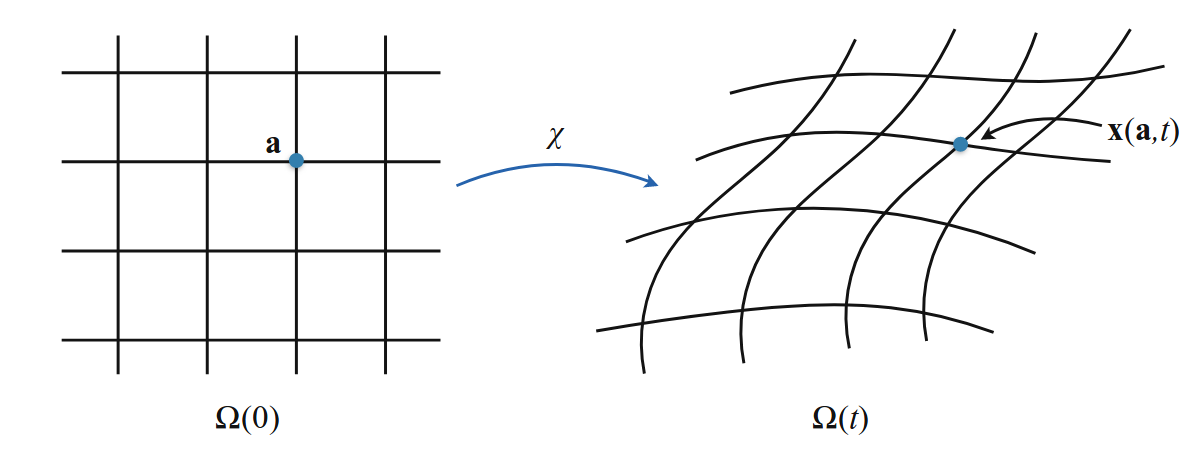
\includegraphics[width=\textwidth]{deform.png}
\centering
\caption{The function $\chi(\bm{a},t)$ maps each fluid element from the initial configuration (material description) to its location in space $\bm{x}$ at time $t$ (Eulerian description) i.e. $\bm{x} = \chi(\bm{a},t)$. From Morozov and Spagnolie~\cite{morozov15a} }
\label{fig:deform}
\end{figure}

\section{Newtonian Fluid Dynamics}
We can make use of two distinct reference frames when describing a continuum fluid. These are the material description and Eulerian description. In the material description we label each fluid element with some label $\bm{a}$ which we choose to be the initial position of the fluid element in space. The independent variables are then associated with each fluid element and time $t$ e.g., for pressure $P(\bm{a},t)$. In contrast, the Eulerian description gives values of independent variables at points in space $\bm{x}$ and time $t$ i.e., $p(\bm{x},t)$. These descriptions are linked by a map $\chi$ from each label $\bm{a}$ to its position $\bm$ at time $t$, $\bm{x} = \chi(\bm{a},t)$. Both descriptions can be seen in Fig~\ref{fig:deform} where the material description appears on the left and the Eulerian description on the right.

We can use these two descriptions to define the important \textit{material derivative}. We define the velocity of a fluid element at $\bm{x}$ as $\bm{u}(\bm{x},t)$. The velocity of a material point specified with label $\bm{a}$ is then
\begin{equation}
\bm{U}(\bm{a},t) = \bm{u}(\bm{x}(\bm{a},t),t)
\end{equation}
where the capital $\bm{U}$ denotes the material desription. Similarly, a scalar such as the pressure of a fluid element is given in each coordinate system as
\begin{equation}
P(\bm{a},t) = p(\bm{x}(\bm{a},t),t).
\end{equation}
Taking a time derivative in the material description gives simply $\partial_t P(\bm{a},t)$ but taking the same derivative in the Eulerian description, we must account for the change of reference frame. Using the chain rule gives
\begin{equation}
\frac{d}{dt}p(\bm{x}(\bm{a},t),t) = \pardev{p}{t} + \pardev{p}{x_i} \pardev{x_i}{t} = (\partial_t + \bm{u} \cdot \nabla) p = \frac{Dp}{Dt}
\end{equation}
where the $x_i$ are components of space and we have used the Einstein convention. We have defined the material derivative as
\begin{equation}
\frac{D}{Dt} \defeq \pardev{}{t} + \bm{u} \cdot \nabla.
\end{equation}
This time derivative ``follows the fluid" in the sense that is the time derivative of a field at a specific fluid element measured in the Eulerian frame. The same material derivative can be used for vector fields as well. This leads to the following form for the acceleration of a fluid element:
\begin{equation}
\frac{D\bm{u}}{Dt} = \pardev{\bm{u}}{t} + \bm{u} \cdot \nabla\bm{u}.
\end{equation} 
\subsection{Mass Conservation}
Since there are no mass sources or sinks, any change in mass in some control volume in the Eulerian frame must be gained or lost through the surface of that control volume. This can be expressed mathematically as
\begin{equation}
\frac{d}{dt}\int_{V_0} \rho(\bm{x},t)dV = -\int_{\partial V_0} \rho(\bm{x},t)\bm{u}(\bm{x},t) \cdot d\bm{A}
\end{equation}



\newpage
In this work we treat the solvent of a viscoelastic fluid as an incompressible fluid with the usual Navier-Stokes momentum and mass conservation equations. These are given by
\begin{equation}\label{eq:momentum_conservation}
\rho \left( \frac{\partial \bm{u}}{\partial t} + \left(\bm{u} \cdot \nabla\right)\bm{u}\right) =
-\nabla p +\eta_s \nabla^2 \bm{u} + \bm{F}^{\mathrm{ext}} + \nabla \cdot \bm{\tau} 
\end{equation}
and
\begin{equation}\label{eq:mass_conservation}
\nabla \cdot \bm{u} = 0,
\end{equation}
where $\rho$ is the density, $\bm{u}$ is the velocity field, $p$ is the pressure, $\eta_s$ is the viscosity of the solvent, $\bm{F}^{\mathrm{ext}}$ is an external force density on the fluid, and $\bm{\tau}$ the so-called extra stress tensor. Here we see that the divergence of the extra stress tensor leads to a forcing term in the momentum conservation equation. 

Although, on the microscopic level, viscoelastic effects are due to the stretching and relaxation of polymers suspended in the solvent, we will be using a continuum model to develop this extra stress tensor in time. The Oldroyd-B model is commonly used to describe viscoelastic flow and is mathematically equivalent to a fluid filled with harmonic spring "dumbells." The Oldroyd-B model provides a constitutive equation for the extra stress tensor which has the form
\begin{equation}\label{eq:short_oldroyd_b}
\overset{\nabla}{\bm{\tau}} = \frac{1}{\lambda_p}\left(2\eta_p\bm{d}- \bm{\tau}\right)
\end{equation}
where $\lambda_p$ and $\eta_p$ are the relaxation time and added viscosity of the polymer solution, respectively, and  
\begin{equation}\label{eq:rate_of_strain}
\bm{d} \defeq \frac{1}{2}\left(\nabla\bm{u} + \nabla \bm{u}^T\right)
\end{equation}
is the rate of strain tensor where $T$ indicates the transpose. The upper-convected time derivative is defined as
\begin{equation}\label{eq:upper_convected_derivative}
\overset{\nabla}{\bm{\tau}} \defeq \frac{\partial \bm{\tau}}{\partial t} + (\bm{u} \cdot \nabla)\bm{\tau} - \bm{\tau} \cdot \nabla\bm{u} -(\nabla\bm{u})^\intercal \cdot \bm{\tau}
\end{equation}
and describes the time evolution of a tensor being transported along a velocity field $\bm{u}$. Use of this time derivative is required so that our constitutive relation Note that it is important that we choose the convention that
\begin{equation}\label{eq:gradient_convention}
(\nabla \bm{u})_{\alpha\beta} \defeq \frac{\partial u_{\beta}}{\partial x_\alpha}
\end{equation}
in order that Eq.~\eqref{eq:upper_convected_derivative} be the correct form. Finally, we may write the constitutive equation as
\begin{equation}\label{eq:full_oldroyd_b}
\frac{\partial \bm{\tau}}{\partial t} + (\bm{u} \cdot \nabla)\bm{\tau}= \left(\bm{\tau} \cdot \nabla\bm{u} +(\nabla\bm{u})^T \cdot \bm{\tau}\right) + \frac{1}{\lambda_p}\left(2\eta_p \bm{d} - \bm{\tau}\right).
\end{equation}
We aim to develop these two equations numerically in order to simulate an Oldroyd-B fluid.